\documentclass[12pt]{article}
\usepackage{vntex}
% \usepackage[english, vietnamese]{babel}
\usepackage{tikz}
\usepackage[left=3.00cm, right=2.00cm, top=2.00cm, bottom=2.00cm]{geometry}
\usepackage[unicode]{hyperref}
\usepackage{amsmath}
\usepackage{amssymb}
\usepackage{graphicx}
\usepackage{a4wide,amssymb,epsfig,latexsym,array,hhline,fancyhdr}
\usepackage[normalem]{ulem}
\usepackage[makeroom]{cancel}
\usepackage{amsthm}
\usepackage{multicol,longtable,amscd}
\usepackage{diagbox}
\usepackage{booktabs}
\usepackage{alltt}
\usepackage[framemethod=tikz]{mdframed}
\usepackage{caption,subcaption}
\usepackage{listings}
\usepackage{color}
\usepackage{lipsum}
\usepackage{setspace}
\usepackage{titling}
\usepackage{multicol}
\usepackage{indentfirst}
\usepackage{float}

\usetikzlibrary{decorations}
\usetikzlibrary{decorations.pathreplacing}
\usetikzlibrary{decorations.pathreplacing,calligraphy}
\usetikzlibrary{arrows.meta}
\usetikzlibrary{quotes}
\usetikzlibrary{intersections}
\usetikzlibrary{calc}

\setstretch{1.15}

\newtheorem{theorem}{Định lý}
\newtheorem{corollary}{Hệ quả}
\newtheorem{lemma}{Bổ đề}
\newtheorem*{remark}{Nhận xét}
\newtheorem{definition}{Định nghĩa}
\newtheorem*{recap}{Tóm lại}


\title{\textbf{Định lý Kuratowski}}
\posttitle{
\par\end{center}
\begin{center}\LARGE(Toán rời rạc)\end{center}
\vskip0.5em}



\author{
    Nguyễn Đức Huy \thanks{K64 Máy tính và Khoa học Thông tin}\\
    Hà Nội \\
    Đại học Khoa học Tự Nhiên \\
    mail@edu
    \and
    Trần Thị Như Quỳnh \thanks{K65 Khoa học Dữ liệu} \\
    Hà Nội \\
    Đại học Khoa học Tự Nhiên \\
    mail@edu
    \and
    Bùi Khánh Duy \thanks{K65 Máy tính và Khoa học Thông tin}\\
    Nghệ An \\
    Đại học Khoa học Tự Nhiên \\
    mail@edu
}

\begin{document}
\begin{titlepage}
    \maketitle
    \begin{abstract}
        Bài viết này giới thiệu các khái niệm và định lý cơ bản trong đồ thị, tập trung vào đồ thị phẳng. Trên nền tảng của những điều cơ bản, chúng tôi phát biểu và trình bày một chứng minh chặt chẽ về định lý Kuratowski, bao gồm điều kiện cần và đủ để có tính chính xác. \footnote{Quyền sao chép một phần hoặc toàn bộ bài viết này cho mục đích sử dụng cá nhân hoặc lớp học được cho phép với điều kiện bản sao không được tạo ra hoặc phân phối vì lợi nhuận hoặc mục đích thương mại và các bản sao đó phải trích dẫn đầy đủ thông báo này trên trang đầu tiên. Các bên thứ ba của bài viết này phải được tôn trọng. Đối với tất cả các mục đích sử dụng khác, hãy liên hệ với chủ sở hữu hoặc các tác giả}
    \end{abstract}
\end{titlepage}

\begin{titlepage}
    \tableofcontents
\end{titlepage}

\section{Mở đầu}

Về tính phẳng của đồ thị, liệu đồ thị có thể được vẽ trên một mặt phẳng theo cách không có cạnh nào cắt nhau hay không,
là một tính chất thú vị cần khảo sát. Với một vài định lý đơn giản, có thể thấy rằng $K_5$ và $K_{3,3}$ là đồ thị không phẳng.
Kuratowski đã sử dụng quan sát gần như dễ dàng này thành một định lý mạnh mẽ cho thấy điều kiện cần và đủ của tính phẳng.
Để chứng minh định lý này, ta cần sử dụng một vài các định lý, hệ quả và bổ đề.
Trong bài viết này, chúng tôi bắt đầu với lý thuyết đồ thị cơ bản, sau đó tới các khái niệm và định lý liên quan đến đồ thị phẳng.
Trong phần cuối cùng, chúng tôi sẽ đưa ra một cách chứng minh định lý Kuratowski.
\section{Phát biểu định lý}

\begin{theorem}[Kuratowski]
    \label{thr:kuratowski}
    Một đồ thị phẳng khi và chỉ khi không chứa bất kỳ đồ thị con nào là subdivision của $K_5$ hoặc $K_{3,3}$
\end{theorem}

\begin{center}
    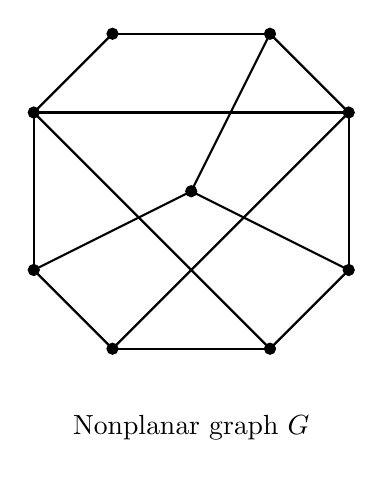
\begin{tikzpicture}
        \draw[black, thick] (0,1) -- (1,0);
        \draw[black, thick] (0,1) -- (2,2);
        \draw[black, thick] (3,4) -- (2,2);
        \draw[black, thick] (3,4) -- (1,4);
        \draw[black, thick] (0,3) -- (1,4);
        \draw[black, thick] (4,3) -- (3,4);
        \draw[black, thick] (1,0) -- (4,3);
        \draw[black, thick] (1,0) -- (3,0);
        \draw[black, thick] (3,0) -- (4,1);
        \draw[black, thick] (3,0) -- (0,3);
        \draw[black, thick] (2,2) -- (4,1);
        \draw[black, thick] (0,1) -- (0,3);
        \draw[black, thick] (4,1) -- (4,3);
        \draw[black, thick] (0,3) -- (4,3);

        \filldraw[black] (1,0) circle (2pt);
        \filldraw[black] (0,1) circle (2pt);
        \filldraw[black] (3,0) circle (2pt);
        \filldraw[black] (4,1) circle (2pt);
        \filldraw[black] (2,2) circle (2pt);
        \filldraw[black] (0,3) circle (2pt);
        \filldraw[black] (4,3) circle (2pt);
        \filldraw[black] (1,4) circle (2pt);
        \filldraw[black] (3,4) circle (2pt);

        \node at (2, -1, 0) {Nonplanar graph $G$};
    \end{tikzpicture}

\end{center}

\begin{center}
    \label{fig:G1}
    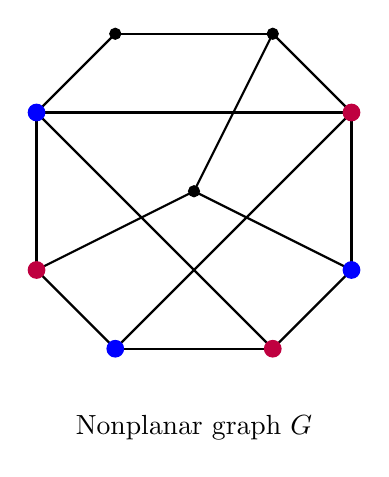
\begin{tikzpicture}
        \draw[black, thick] (0,1) -- (1,0);
        \draw[black, thick] (0,1) -- (2,2);
        \draw[black, thick] (3,4) -- (2,2);
        \draw[black, thick] (3,4) -- (1,4);
        \draw[black, thick] (0,3) -- (1,4);
        \draw[black, thick] (4,3) -- (3,4);
        \draw[black, thick] (1,0) -- (4,3);
        \draw[black, thick] (1,0) -- (3,0);
        \draw[black, thick] (3,0) -- (4,1);
        \draw[black, thick] (3,0) -- (0,3);
        \draw[black, thick] (2,2) -- (4,1);
        \draw[black, thick] (0,1) -- (0,3);
        \draw[black, thick] (4,1) -- (4,3);
        \draw[black, thick] (0,3) -- (4,3);

        \filldraw[blue] (1,0) circle (3pt);
        \filldraw[purple] (0,1) circle (3pt);
        \filldraw[purple] (3,0) circle (3pt);
        \filldraw[blue] (4,1) circle (3pt);
        \filldraw[black] (2,2) circle (2pt);
        \filldraw[blue] (0,3) circle (3pt);
        \filldraw[purple] (4,3) circle (3pt);
        \filldraw[black] (1,4) circle (2pt);
        \filldraw[black] (3,4) circle (2pt);

        \node at (2,-1,0) {Nonplanar graph $G$};
    \end{tikzpicture}

\end{center}

\begin{center}
    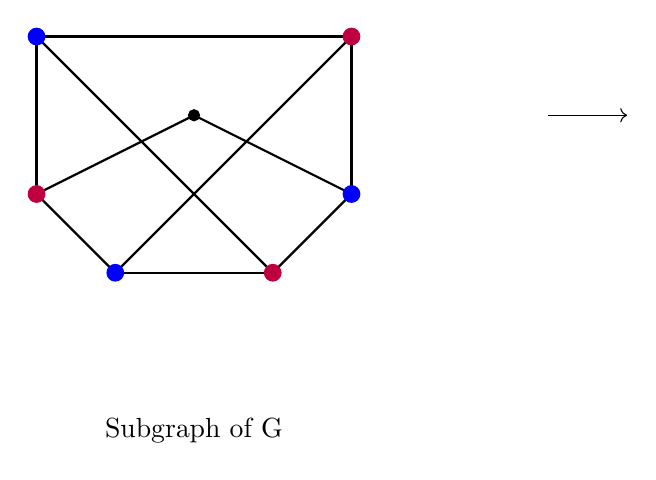
\begin{tikzpicture}
        \draw[black, thick] (0,1) -- (1,0);
        \draw[black, thick] (1,0) -- (4,3);
        \draw[black, thick] (1,0) -- (3,0);
        \draw[black, thick] (3,0) -- (4,1);
        \draw[black, thick] (3,0) -- (0,3);
        \draw[black, thick] (0,1) -- (0,3);
        \draw[black, thick] (4,1) -- (4,3);
        \draw[black, thick] (0,3) -- (4,3);
        \draw[black, thick] (0,1) -- (2,2);
        \draw[black, thick] (2,2) -- (4,1);
        \filldraw[blue] (1,0) circle (3pt);
        \filldraw[purple] (0,1) circle (3pt);
        \filldraw[purple] (3,0) circle (3pt);
        \filldraw[blue] (4,1) circle (3pt);
        \filldraw[blue] (0,3) circle (3pt);
        \filldraw[purple] (4,3) circle (3pt);
        \filldraw[black] (2,2) circle (2pt);
        \draw [-{To}] (6.5, 2) -- (7.5, 2);
        \node at (2,-2,0) {Subgraph of G};
    \end{tikzpicture}
    \hspace{2cm}
    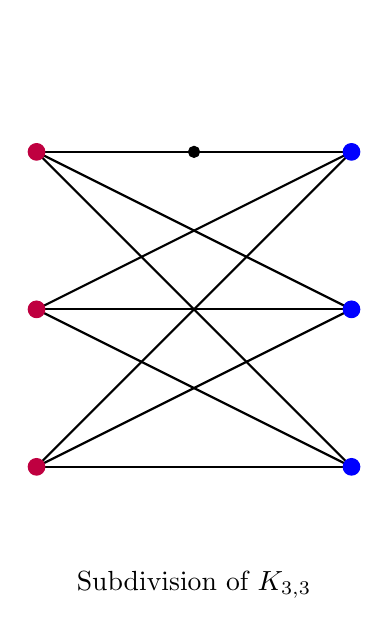
\begin{tikzpicture}
        \draw[black, thick] (8,-0.5) -- (12,-0.5);
        \draw[black, thick] (8,-0.5) -- (12,1.5);
        \draw[black, thick] (8,-0.5) -- (12,3.5);
        \draw[black, thick] (8,1.5) -- (12,-0.5);
        \draw[black, thick] (8,1.5) -- (12,1.5);
        \draw[black, thick] (8,1.5) -- (12,3.5);
        \draw[black, thick] (8,3.5) -- (12,-0.5);
        \draw[black, thick] (8,3.5) -- (12,1.5);
        \draw[black, thick] (8,3.5) -- (12,3.5);
        \filldraw[white] (10,5) circle (2pt);
        \filldraw[black] (10,3.5) circle (2pt);
        \filldraw[blue] (12,-0.5) circle (3pt);
        \filldraw[purple] (8,-0.5) circle (3pt);
        \filldraw[blue] (12,1.5) circle (3pt);
        \filldraw[purple] (8,1.5) circle (3pt);
        \filldraw[blue] (12,3.5) circle (3pt);
        \filldraw[purple] (8,3.5) circle (3pt);
        \node at (10,-2,0) {Subdivision of $K_{3,3}$};
    \end{tikzpicture}
\end{center}
\section{Định lý Kuratowski}
Năm 1930, Kuratowski công bố định lý đưa ra một điều kiện cần và đủ cho tính phẳng.
\begin{theorem}[Kuratowski]
    \label{thr:kuratowski}
    Một đồ thị phẳng khi và chỉ khi không chứa bất kỳ đồ thị con nào là đồ thị phân chia của $K_5$ hoặc $K_{3,3}$
\end{theorem}
\begin{figure}[H]
    \centering
    \begin{minipage}{0.05\textwidth}

    \end{minipage}
    \hfill
    \begin{minipage}{0.55\textwidth}

        \begin{tikzpicture}
            \draw[black, thick] (0,1) -- (1,0);
            \draw[black, thick] (0,1) -- (2,2);
            \draw[black, thick] (3,4) -- (2,2);
            \draw[black, thick] (3,4) -- (1,4);
            \draw[black, thick] (0,3) -- (1,4);
            \draw[black, thick] (4,3) -- (3,4);
            \draw[black, thick] (1,0) -- (4,3);
            \draw[black, thick] (1,0) -- (3,0);
            \draw[black, thick] (3,0) -- (4,1);
            \draw[black, thick] (3,0) -- (0,3);
            \draw[black, thick] (2,2) -- (4,1);
            \draw[black, thick] (0,1) -- (0,3);
            \draw[black, thick] (4,1) -- (4,3);
            \draw[black, thick] (0,3) -- (4,3);

            \filldraw[black] (1,0) circle (2pt);
            \filldraw[black] (0,1) circle (2pt);
            \filldraw[black] (3,0) circle (2pt);
            \filldraw[black] (4,1) circle (2pt);
            \filldraw[black] (2,2) circle (2pt);
            \filldraw[black] (0,3) circle (2pt);
            \filldraw[black] (4,3) circle (2pt);
            \filldraw[black] (1,4) circle (2pt);
            \filldraw[black] (3,4) circle (2pt);

            \node at (2, -1, 0) {Đồ thị không phẳng $G$};
        \end{tikzpicture}

    \end{minipage}
    \hfill
    \begin{minipage}{0.325\textwidth}
        \label{fig:G1}
        \begin{tikzpicture}
            \draw[black, thick] (0,1) -- (1,0);
            \draw[black, thick] (0,1) -- (2,2);
            \draw[black, thick] (3,4) -- (2,2);
            \draw[black, thick] (3,4) -- (1,4);
            \draw[black, thick] (0,3) -- (1,4);
            \draw[black, thick] (4,3) -- (3,4);
            \draw[black, thick] (1,0) -- (4,3);
            \draw[black, thick] (1,0) -- (3,0);
            \draw[black, thick] (3,0) -- (4,1);
            \draw[black, thick] (3,0) -- (0,3);
            \draw[black, thick] (2,2) -- (4,1);
            \draw[black, thick] (0,1) -- (0,3);
            \draw[black, thick] (4,1) -- (4,3);
            \draw[black, thick] (0,3) -- (4,3);

            \filldraw[blue] (1,0) circle (3pt);
            \filldraw[purple] (0,1) circle (3pt);
            \filldraw[purple] (3,0) circle (3pt);
            \filldraw[blue] (4,1) circle (3pt);
            \filldraw[black] (2,2) circle (2pt);
            \filldraw[blue] (0,3) circle (3pt);
            \filldraw[purple] (4,3) circle (3pt);
            \filldraw[black] (1,4) circle (2pt);
            \filldraw[black] (3,4) circle (2pt);

            \node at (2,-1,0) {Đồ thị không phẳng $G$};
        \end{tikzpicture}

    \end{minipage}
\end{figure}

\begin{figure}[H]
    \centering

    \begin{tikzpicture}
        \draw[black, thick] (0,1) -- (1,0);
        \draw[black, thick] (1,0) -- (4,3);
        \draw[black, thick] (1,0) -- (3,0);
        \draw[black, thick] (3,0) -- (4,1);
        \draw[black, thick] (3,0) -- (0,3);
        \draw[black, thick] (0,1) -- (0,3);
        \draw[black, thick] (4,1) -- (4,3);
        \draw[black, thick] (0,3) -- (4,3);
        \draw[black, thick] (0,1) -- (2,2);
        \draw[black, thick] (2,2) -- (4,1);
        \filldraw[blue] (1,0) circle (3pt);
        \filldraw[purple] (0,1) circle (3pt);
        \filldraw[purple] (3,0) circle (3pt);
        \filldraw[blue] (4,1) circle (3pt);
        \filldraw[blue] (0,3) circle (3pt);
        \filldraw[purple] (4,3) circle (3pt);
        \filldraw[black] (2,2) circle (2pt);
        \draw [-{To}] (6.5, 2) -- (7.5, 2);
        \node at (2,-2,0) {Đồ thị con của $G$};
    \end{tikzpicture}
    \hspace{2cm}
    \begin{tikzpicture}
        \draw[black, thick] (8,-0.5) -- (12,-0.5);
        \draw[black, thick] (8,-0.5) -- (12,1.5);
        \draw[black, thick] (8,-0.5) -- (12,3.5);
        \draw[black, thick] (8,1.5) -- (12,-0.5);
        \draw[black, thick] (8,1.5) -- (12,1.5);
        \draw[black, thick] (8,1.5) -- (12,3.5);
        \draw[black, thick] (8,3.5) -- (12,-0.5);
        \draw[black, thick] (8,3.5) -- (12,1.5);
        \draw[black, thick] (8,3.5) -- (12,3.5);
        \filldraw[white] (10,5) circle (2pt);
        \filldraw[black] (10,3.5) circle (2pt);
        \filldraw[blue] (12,-0.5) circle (3pt);
        \filldraw[purple] (8,-0.5) circle (3pt);
        \filldraw[blue] (12,1.5) circle (3pt);
        \filldraw[purple] (8,1.5) circle (3pt);
        \filldraw[blue] (12,3.5) circle (3pt);
        \filldraw[purple] (8,3.5) circle (3pt);
        \node at (10,-2,0) {Đồ thị phân chia của $K_{3,3}$};
    \end{tikzpicture}
\end{figure}

Để chứng minh định lý này, ta cần chứng minh một số bổ đề cần thiết.

\section{Sơ bộ}
\subsection{Tính chất của đồ thị con và subdivision}

\begin{corollary}
    Đồ thị con của đồ thị phẳng là đồ thị phẳng
\end{corollary}

\begin{proof}
    Nếu $G$ là đồ thị phẳng, nghĩa là tồn tại một biểu diễn phẳng của $G$. Với mọi đồ thị con
    $H$ của $G$, ta có thể tìm đươc các đỉnh và cạnh của $H$ trong biểu diễn phẳng của $G$.
    Từ đó, ta dựng được một biểu diễn phẳng của $H$.
\end{proof}


\begin{corollary}
    Subdivision của một đồ thị không phẳng là một đồ thị không phẳng.\end{corollary}
\begin{proof}
    Ai biết đâu.
\end{proof}

\subsection{2-Connected Graphs and their Properties}
\begin{definition}
    A graph is 2-connected if it cannot be separated into two components by removing a single vertex
\end{definition}
\begin{center}
    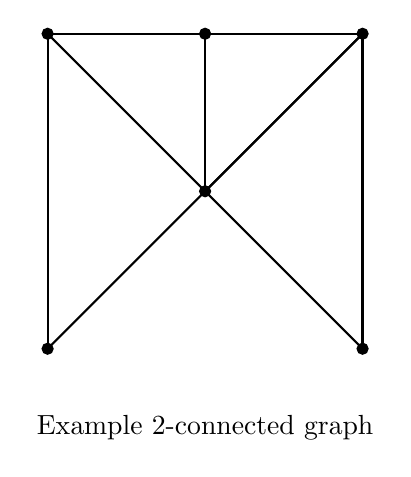
\begin{tikzpicture}
        \draw[black, thick] (0,0) -- (0,4);
        \draw[black, thick] (0,0) -- (4,4);
        \draw[black, thick] (4,0) -- (4,4);
        \draw[black, thick] (2,2) -- (4,4);
        \draw[black, thick] (2,2) -- (2,4);
        \draw[black, thick] (0,4) -- (4,4);
        \draw[black, thick] (0,4) -- (4,0);
        \foreach \x/\y in {0/0, 0/4, 2/2, 2/4, 4/0, 4/4} {
                \filldraw[black] (\x,\y) circle (2pt);
            }
        \node at (2,-1,0) {Example 2-connected graph};
    \end{tikzpicture}
    \hspace{2cm}
    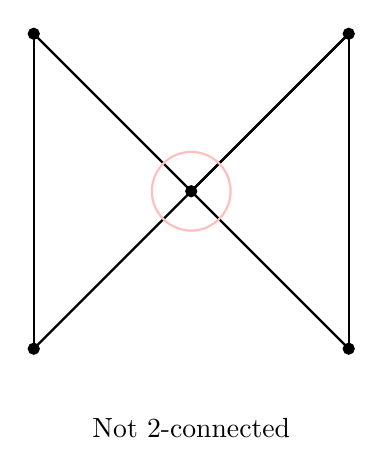
\begin{tikzpicture}
        \draw[black, thick] (0,0) -- (0,4);
        \draw[black, thick] (0,0) -- (4,4);
        \draw[black, thick] (4,0) -- (4,4);
        \draw[black, thick] (2,2) -- (4,4);
        \draw[black, thick] (0,4) -- (4,0);
        \draw[pink, thick] (2,2) circle (0.5);
        \foreach \x/\y in {0/0, 0/4, 2/2, 4/0, 4/4} {
                \filldraw[black] (\x,\y) circle (2pt);
            }
        \node at (2,-1,0) {Not 2-connected};
    \end{tikzpicture}
\end{center}
\begin{theorem}
    Mọi cặp đỉnh trong đồ thị 2-connected đều nằm trên cùng một chu trình.
    \begin{proof}
        Quy nạp:

        Trường hợp cơ bản: $u$ kề $v$
        \begin{center}
            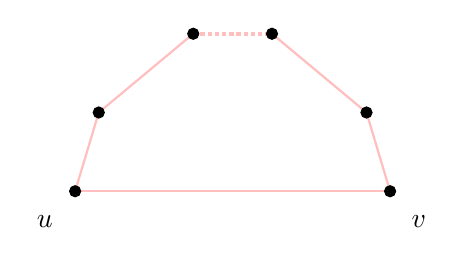
\begin{tikzpicture}
                \draw[pink, thick] (0,0) -- (0.3,1);
                \draw[pink, thick] (0.3,1) -- (1.5,2);
                \draw[densely dotted, pink, ultra thick] (1.5,2) -- (2.5,2);
                \draw[pink, thick] (2.5,2) -- (3.7,1);
                \draw[pink, thick] (3.7,1) -- (4,0);
                \draw[pink, thick] (0,0) -- (4,0);
                \node at (0,0,1) {$u$};
                \node at (4.75,0,1) {$v$};
                \filldraw[black] (0,0) circle (2pt);
                \filldraw[black] (0.3,1) circle (2pt);
                \filldraw[black] (1.5,2) circle (2pt);
                \filldraw[black] (2.5,2) circle (2pt);
                \filldraw[black] (3.7,1) circle (2pt);
                \filldraw[black] (4,0) circle (2pt);
            \end{tikzpicture}
        \end{center}
        Quy nạp: $u,v$ có khoảng cách $d+1$
        \begin{center}
            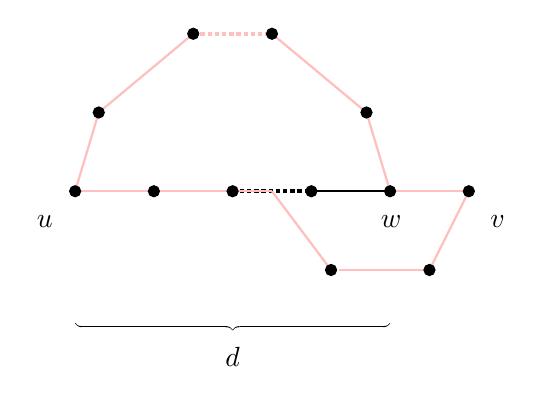
\begin{tikzpicture}
                \draw[pink, thick] (0,0) -- (0.3,1);
                \draw[pink, thick] (0.3,1) -- (1.5,2);
                \draw[densely dotted, pink, ultra thick] (1.5,2) -- (2.5,2);
                \draw[pink, thick] (2.5,2) -- (3.7,1);
                \draw[pink, thick] (3.7,1) -- (4,0);
                \draw[pink, thick] (0,0) -- (2,0);
                \draw[black, thick] (3,0) -- (4,0);
                \draw[pink, thick] (4,0) -- (5,0);
                \draw[densely dotted, black, ultra thick] (2,0) -- (3,0);
                \draw[pink, thick] (2.5,0) -- (3.25,-1);
                \draw[pink, thick] (3.35,-1) -- (4.5,-1);
                \draw[pink, thick] (5,0) -- (4.5,-1);
                \draw[pink, thick] (2,0) -- (2.5,0);

                \node at (0,0,1) {$u$};
                \node at (5.75,0,1) {$v$};
                \node at (4.4,0,1) {$w$};
                \filldraw[black] (0,0) circle (2pt);
                \filldraw[black] (0.3,1) circle (2pt);
                \filldraw[black] (1.5,2) circle (2pt);
                \filldraw[black] (2.5,2) circle (2pt);
                \filldraw[black] (3.7,1) circle (2pt);
                \filldraw[black] (1,0) circle (2pt);
                \filldraw[black] (2,0) circle (2pt);
                \filldraw[black] (3,0) circle (2pt);
                \filldraw[black] (4,0) circle (2pt);
                \filldraw[black] (5,0) circle (2pt);
                \filldraw[black] (3.25,-1) circle (2pt);
                \filldraw[black] (4.5,-1) circle (2pt);

                \draw [decorate, decoration = {calligraphic brace, mirror, raise=5pt}] (0,-1.5) --  (4,-1.5) node[pos=0.5,below=10pt,black]{$d$};
            \end{tikzpicture}
        \end{center}
    \end{proof}
\end{theorem}
\section{Chứng minh định lý}
$(\Rightarrow)$  Nếu đồ thị $G$ chứa đồ thị con là đồ thị phân chia của $K_5$ hoặc $K_{3,3}$ thì $G$ không phẳng. \\

\begin{proof}
    Ta có:
    \begin{itemize}
        \item Đồ thị phân chia của đồ thị không phẳng thì không phẳng

        \item Nếu một đồ thị con không phẳng thì đồ thị không phẳng

        \item Nếu một đồ thị con của đồ thị $G$ là đồ thị phân chia của đồ thị không phẳng thì $G$ không phẳng
    \end{itemize}
    \begin{lemma}
        $K_{3,3}$ is không phẳng
    \end{lemma}

    \begin{proof}
        Chúng ta sẽ chứng minh bằng phản chứng.

        Giả sử tồn tại một biểu diễn phẳng của $K_{3,3}$. Trong đồ thị phân đôi đơn, chiều dài nhỏ nhất của chu trình là 4, nghĩa là với mọi $f \in F(K_{3,3})$
        $$deg(f) \geq 4$$
        Lại có $$\sum_{f \in F(K_{3,3})}deg(f) = 2\epsilon$$
        \begin{figure}[H]
            \begin{minipage}{0.3\textwidth}
                \begin{eqnarray*}
                    \nu-\epsilon+\phi& = &2 \\
                    6-\epsilon+\phi& = & 2\\
                    6-9+\phi& = & 2\\
                    \phi& = & 5\\
                \end{eqnarray*}
            \end{minipage}
            \hfill
            \begin{minipage}{0.35\textwidth}
                \centering
                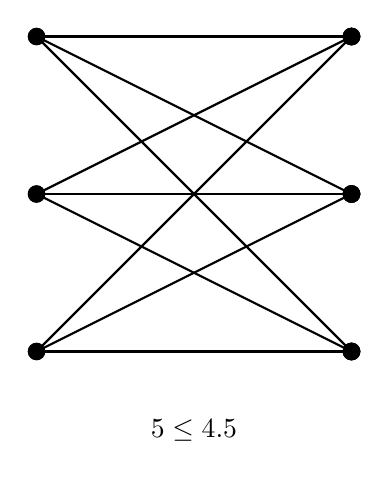
\begin{tikzpicture}
                    \foreach \x/\y in {0/1, 0/3, 0/5} {
                            \filldraw[black] (\x,\y) circle (3pt);
                            \foreach \z/\t in {4/1, 4/3, 4/5} {
                                    \filldraw[black] (\z,\t) circle (3pt);
                                    \draw[black, thick] (\x,\y) -- (\z,\t);
                                }
                        }
                    \node at (2,0,0) {$5 \leq 4.5$};
                \end{tikzpicture}
            \end{minipage}
            \hfill
            \begin{minipage}{0.3\textwidth}
                \centering
                % No 3 edge faces
                \begin{eqnarray*}
                    4\phi& \leq &2\epsilon\\
                    4\phi& \leq & 2 \times 9\\
                    \phi& \leq & 4.5
                \end{eqnarray*}
            \end{minipage}
        \end{figure}
    \end{proof}

    \begin{lemma}
        $K_5$ is không phẳng
    \end{lemma}
    \begin{proof}
        Giả sử tồn tại một biểu diễn phẳng của $K_{3,3}$. Trong đồ thị phân đôi đơn, chiều dài nhỏ nhất của chu trình là 4, nghĩa là với mọi $f \in F(K_{3,3})$
        $$deg(f) \geq 3$$
        Lại có $$\sum_{f \in F(K_{3,3})}deg(f) = 2\epsilon$$
        \begin{figure}[H]
            \begin{minipage}{0.3\textwidth}
                \begin{eqnarray*}
                    \nu-\epsilon+\phi& = &2 \\
                    5-\epsilon+\phi& = & 2\\
                    5-10+\phi& = & 2\\
                    \phi& = & 7\\
                \end{eqnarray*}
            \end{minipage}
            \hfill
            \begin{minipage}{0.35\textwidth}
                \centering
                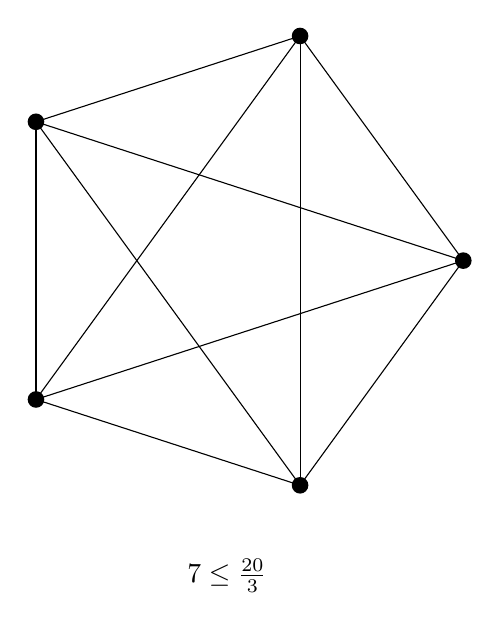
\begin{tikzpicture}
                    \foreach \i in {1, 2, 3, 4, 5}
                    \fill[black] (\i*360/5:3) coordinate (5\i) circle(3 pt)
                    \ifnum \i>1 foreach \j in {\i,...,1}{(5\i) edge (5\j)} \fi;

                    \node at (0,-4,0) {$7 \leq \frac{20}{3}$};
                \end{tikzpicture}
            \end{minipage}
            \hfill
            \begin{minipage}{0.3\textwidth}
                \centering
                \begin{eqnarray*}
                    3\phi& \leq &2\epsilon\\
                    3\phi& \leq & 2 \times 10\\
                    \phi& \leq & \frac{30}{3}
                \end{eqnarray*}
            \end{minipage}
        \end{figure}
    \end{proof}
    \begin{recap}
    \end{recap}
    $K_5$ và $K_{3,3}$ là không phẳng

    $\Rightarrow$ Tất cả subdivisions của chúng đều không phẳng

    $\Rightarrow$ Nếu đồ thị $G$ chứa đồ thị con là đồ thị phân chia của $K_5$ hoặc $K_{3,3}$ thì G không phẳng \\

\end{proof}
$(\Leftarrow)$ Nếu đồ thị $G$ không phẳng thì $G$ chứa đồ thị phân chia của $K_5$ hoặc $K_{3,3}$
\begin{proof}
    Giả sử tồn tại đồ thị không phẳng mà không chứa đồ thị con là subdivisions của $K_5$ hoặc $K_{3,3}$.

    Cho $G$ là đồ thị có \textit{ít cạnh nhất}. Khi loại bỏ một cạnh bất kì của $G$ thì ta được đồ thị \textit{phẳng}.

    Giả sử $G$ có nhiều thành phần liên thông, dễ thấy $G$ phải có một thành phần liên thông không phẳng. Gọi thành phần liên thông đó là $K$.
    Rõ ràng $\epsilon(K) \leq \epsilon(G)$ và $K$ không chứa $K_5$ và $K_{3,3}$. Khi $K$ ít cạnh hơn $G$, $G$ sẽ không phải đồ thị không phẳng \textit{ít cạnh nhất}, mâu thuẫn, do đó $\epsilon(K) = \epsilon(G)$
    và các thành phần liên thông khác $K$ của $G$ đều chỉ gồm đỉnh cô lập. Không mất tính tổng quát, giả sử $G$ liên thông.

    \begin{enumerate}
        \item $G$ là 2-connected
              \begin{proof}
                  \begin{figure}[H]
                      \centering
                      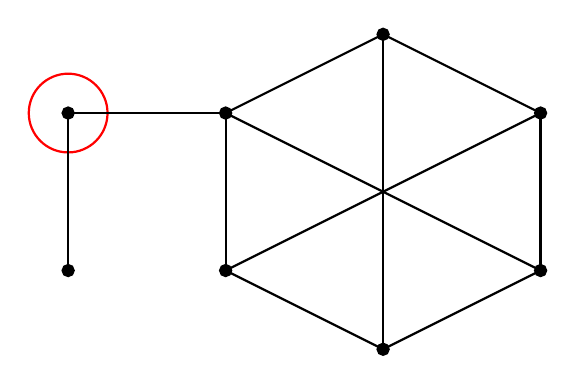
\begin{tikzpicture}
                          \draw[red, thick] (-2,3) circle (0.5);
                          \foreach \x/\y in {0/1, 2/0, 4/1, 0/3, 4/3, 2/4} {
                                  \filldraw[black, thick] (\x,\y) circle (2pt);
                                  \draw[black, thick] (2,2) -- (\x,\y);
                              }
                          \filldraw[black, thick] (-2,3) circle (2pt);
                          \filldraw[black, thick] (-2,1) circle (2pt);

                          \draw[black, thick] (0,1) -- (2,0);
                          \draw[black, thick] (2,0) -- (4,1);
                          \draw[black, thick] (4,1) -- (4,3);
                          \draw[black, thick] (0,3) -- (0,1);
                          \draw[black, thick] (4,3) -- (2,4);
                          \draw[black, thick] (2,4) -- (0,3);

                          \draw[black, thick] (-2,1) -- (-2,3);
                          \draw[black, thick] (-2,3) -- (0,3);

                      \end{tikzpicture}
                  \end{figure}
                  %   Đầu tiên, ta chỉ ra $G$ 1-connected (liên thông). Giả sử $G$ không liên thông, và không phẳng.
                  %   Vì $G$ là đồ thị không phẳng \textit{ít cạnh nhất} nên các thành phần của nó là phẳng. Không mất tính tổng quát, giả sử G có 2 thành phần liên thông là $G_1$ và $G_2$.
                  %   Bởi vì $G_1$ và $G_2$ cùng phẳng, ta có thể thêm biểu diễn phẳng của $G_1$ vào một trong các diện biểu diễn phẳng của $G_2$ (ví dụ diện vô hạn), cho ta biểu diễn phẳng của $G$. Vô lý.

                  Vì $G$ liên thông nên $\kappa(G) \geq 1$. Giả sử $\kappa(G) = 1$, theo định nghĩa, tồn tại đỉnh $v$ sao cho $G -v$ không liên thông.
                  Không mất tính tổng quát, giả sử $G-v$ có 2 thành phần liên thông $H_1$ và $H_2$.
                  Ta có $H_1 \cup v$ và $H_2 \cup v$ đều phẳng vì tính cực tiểu của $G$.
                  Trong biểu diễn phẳng của chúng, ta có thể tìm một diện $f$ mà biên chứa đỉnh $v$.
                  Với phép chiếu lập thể, ta có thể thu được biểu diễn phẳng của $H_1 \cup v$ và $H_2 \cup v$ mà $v$ nằm trên đường biên của diện không bị chặn.
                  Bằng cách đặt điểm ở vô cùng.
                  Sau đó, ta gộp $H_1 \cup v$ và $H_2 \cup v$ bằng cách hợp nhất $v$ và thu được một biểu diễn phẳng của G. Vô lý.
                  \begin{figure}[H]
                      \centering
                      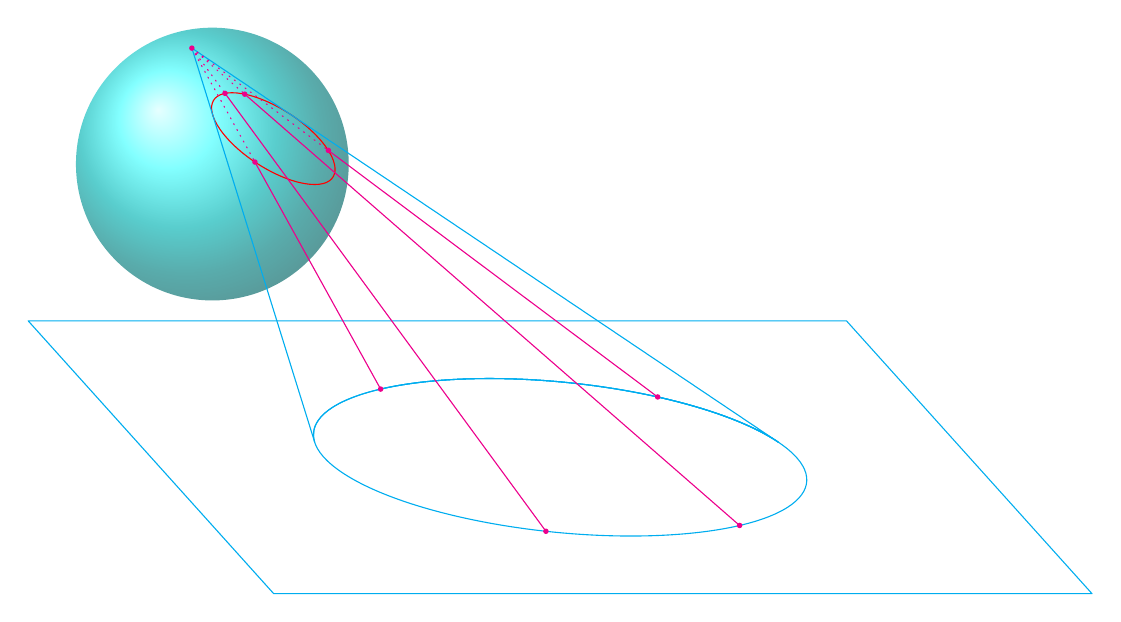
\begin{tikzpicture}[line join=round, line cap=round, >=stealth]%Hinh nón
                          \def\a{1}% Bán trục lớn
                          \def\b{\a/3}% Bán trục bé
                          \pgfmathsetmacro{\h}{sqrt(3)*\a}% Chiều cao
                          \pgfmathsetmacro{\t}{asin(\b/\h)}
                          \shade[ball color=cyan,opacity=0.65](-\h*0.75,0.15*\h)circle(\h);
                          \begin{scope}[xslant=-0.9,magenta]
                              \coordinate (M) at ({\a*cos(\t)}, {\b*sin(\t)});
                              \coordinate (N) at ({-\a*cos(\t)}, {\b*sin(\t)});
                              \path(0,0)coordinate(O)(\a,0)coordinate(A)(-\a,0)coordinate(B);
                              \path (0,\h)coordinate(S)(intersection of A--B and S--N)coordinate(N');
                              \pgfmathsetmacro{\s}{0.5*atan((\h-\b*sin(\t))/(\a*cos(\t)))}
                              \path([rotate around ={{\s}:(N')}]A)coordinate(K)(intersection of N'--K and S--O)coordinate(H);
                              \draw[name path=mot,red] let \p1 =($(O)-(H)$)in(H) circle({veclen(\x1,\y1)});
                              \draw[shift={(0,-2*\h)},scale=3,cyan] ({\a*cos(\t)}, {\b*sin(\t)}) arc(\t:{180-\t}:{\a} and {\b})--(0,\h);
                              \draw[shift={(0,-2*\h)},scale=3,cyan] ({\a*cos(\t)}, {\b*sin(\t)}) arc(\t:360+\t:{\a} and {\b})--(0,\h);
                              \foreach \m[count=\j] in{120,50}{
                                      \draw[shift={(0,-2*\h)},cyan,scale=3] ({\a*cos(\t)}, {\b*sin(\t)}) arc(\t:\m:{\a} and {\b})coordinate(v\j);
                                      \path[name path =hai](v\j)--(0,\h);
                                      \path[name intersections ={of= mot and hai,by={m1\j,n1\j}}];
                                  }
                              \foreach \m[count=\j] in{250,300}{
                                      \path[shift={(0,-2*\h)},scale=3] ({\a*cos(\t)}, {\b*sin(\t)}) arc(\t:\m:{\a} and {\b})coordinate(u\j);
                                      \path[name path =hai](u\j)--(0,\h);
                                      \path[name intersections ={of= mot and hai,by={m2\j,n2\j}}];
                                  }
                              \draw[cyan](-3*\h,-3*\h)rectangle(3*\h,-\h);
                          \end{scope}
                          \draw[dotted,magenta](S)--(n11)(S)--(n12)(S)--(m21)(S)--(m22);
                          \draw[magenta](v1)--(n11)(v2)--(n12)(u1)--(m21)(u2)--(m22);
                          \foreach \d in{v1,S,v2,n11,n12,u1,u2,m21,m22}
                          \fill[magenta](\d)circle(1pt);
                      \end{tikzpicture}
                      \caption*{Ví dụ phép chiếu lập thể từ mặt cầu đến mặt phẳng }
                  \end{figure}
                  Vậy, nếu $G$ là đồ thị không phẳng cực tiểu thì $G$ 2-connected.

              \end{proof}

        \item Nếu $G$ là đồ thị không phẳng \textit{ít cạnh nhất} và $uv$ là một cạnh của $G$ thì $G-uv$ 2-connected
              \begin{proof}
                  Vì $G$ 2-connected nên $\kappa(G) \geq 2$. Giả sử $\kappa(G) =2$ thì tồn tại 2 đỉnh $x,y$ sao cho $G-\{x,y\}$ không liên thông.
                  Gọi các thành phần liên thông của $G-\{x,y\}$ là $H_1, H_2, \ldots,H_k$. Xây dựng tập $M_1,M_2,\ldots,M_k$ trọng đó $M_i=H_i \cup \{x,y\} +xy$.
                  Ta sẽ chỉ ra tồn tại $M_j (1 \geq j \geq k)$ không phẳng.

                  Giả sử tất cả $M_i (1 \geq i \geq k)$ đều phẳng, do đó tồn tại biểu diễn phẳng của mỗi chúng. Với phép chiếu lập thể, ta luôn có một biểu phẳng sao cho $xy$ là biên của diện vô hạn.
                  Vì $\{x,y\}$ và $xy$ là phân chung duy nhất của các $M_i$, do đó, ta có thể hợp nhất biểu diễn phẳng của chúng, thu được biểu diễn phẳng của $G+xy$.
                  Nghĩa là $G+xy$ phẳng, nên $G$ cũng phẳng. Vô lý, do đó tồn tại $M_j (1 \geq j \geq k)$ không phẳng.

                  Giả sử $H_p (1 \geq p \geq k)$ là một thành phần liên thông của $G$.
                  Nếu trong 2 đỉnh $x,y$ không có đỉnh nào nổi với $H_p$, khi đó, $H_p$ là một thành phần liên thông, hay $G$ không liên thông, vô lý.
                  Nếu trong 2 đỉnh $x,y$ có một đỉnh nối tới $H_p$, giả sử $x$, thì khi xóa đỉnh $x$, $G-x$ không còn liên thông, hay $\kappa(G)=1$, vô lý.
                  Vậy cả $x$ và $y$ đều có cạnh nối tới $H_p$ hay có ít nhất 2 cạnh từ $\{x,y\}$ nối đến $H_p$

                  Ta có:
                  \begin{eqnarray*}
                      \epsilon(G)& \geq &\epsilon(H_j+\{x,y\}) + \epsilon(H_p +\{x,y\}) \\
                      & \geq & \epsilon(H_j+\{x,y\}) + 2\\
                      & > & \epsilon(H_j+\{x,y\}) + 1 \\
                      & = & \epsilon(H_j+\{x,y\} + xy) = \epsilon(M_j)
                  \end{eqnarray*}
                  Cuối cùng thì $\epsilon(M_j) < \epsilon(G)$. Vì $G$ là đồ thị ít cạnh nhất không chứa đồ thị phân chia $K_5$ và $K_{3,3}$, $M_j$ không phẳng và ít cạnh hơn $G$, nên $M_j$ phải chứa đồ thị phân chia của $K_5$ hoặc $K_{3,3}$.
                  Suy ra $M_j$ không phải đồ thị con của $G$.
                  Lại có $M_j -xy$ là đồ thị con của $G$ nghĩa là $G$ không chứa cạnh $xy$.
                  Ta hợp nhất $M_j-xy$ với $M_p-xy$ bằng cách hợp nhất đỉnh $x$ và đỉnh $y$, ta thu được một đồ thị con của $G$.
                  Do $M_p -xy$ liên thông nên tồn tại một path giữa $x$ và $y$, kết hợp path này với $M_j-xy$ ta được một đồ thị phân chia của  $K_5$ hoặc $K_{3,3}$.
                  \begin{figure}[H]
                      \centering
                      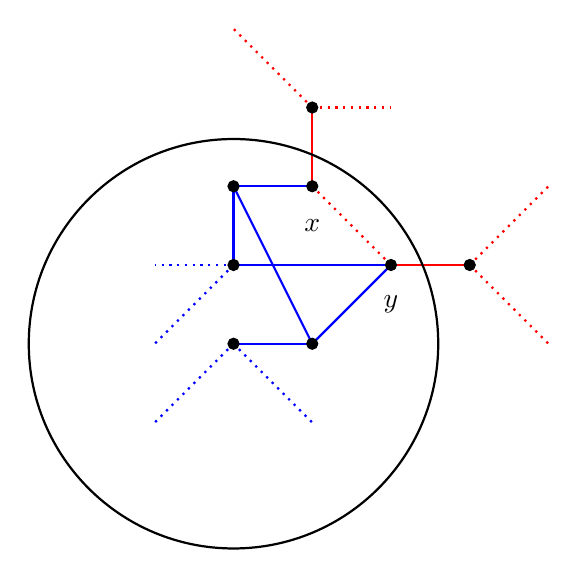
\begin{tikzpicture}
                          \node at (0,0.5,0){$x$};
                          \node at (1,-0.5,0){$y$};
                          \draw[blue, thick] (0, -1) -- (-1,1);
                          \draw[blue, thick] (-1, 0) -- (1,0);
                          \draw[blue, thick] (0, -1) -- (-1,-1);
                          \draw[blue, thick] (0, 1) -- (-1,1);
                          \draw[blue, thick] (-1, 0) -- (-1,1);
                          \draw[blue, thick] (1, 0) -- (0,-1);
                          \draw[red, thick] (1, 0) -- (2,0);
                          \draw[red, thick] (0, 1) -- (0,2);
                          \draw[black, thick] (-1,-1) circle (2.6);
                          \draw[dotted, red, thick] (0, 1) -- (1,0);
                          \draw[dotted, red, thick] (2, 0) -- (3,1);
                          \draw[dotted, red, thick] (2, 0) -- (3,-1);
                          \draw[dotted, red, thick] (0, 2) -- (1,2);
                          \draw[dotted, red, thick] (0, 2) -- (-1,3);
                          \draw[dotted, blue, thick] (-1, 0) -- (-2,0);
                          \draw[dotted, blue, thick] (-1, 0) -- (-2,-1);
                          \draw[dotted, blue, thick] (-1, -1) -- (-2,-2);
                          \draw[dotted, blue, thick] (-1, -1) -- (0,-2);
                          \filldraw[black] (-1,1) circle (2pt);
                          \filldraw[black] (0,-1) circle (2pt);
                          \filldraw[black] (0,1) circle (2pt);
                          \filldraw[black] (1,0) circle (2pt);
                          \filldraw[black] (2,0) circle (2pt);
                          \filldraw[black] (-1,0) circle (2pt);
                          \filldraw[black] (-1,-1) circle (2pt);
                          \filldraw[black] (0,2) circle (2pt);
                      \end{tikzpicture}
                      \caption*{\textcolor{blue}{Xanh}: $M_j-xy$ \\ \textcolor{red}{Đỏ}: $M_p-xy$}
                  \end{figure}


                  Dẫn đến $G$ chứa đồ thị phân chia của $K_5$ hoặc $K_{3,3}$. Vô lý

                  $\Rightarrow \kappa(G) \geq 3$ hay $G$ 3-connected.
              \end{proof}
              Tiếp theo, ta sẽ chỉ ra với mọi cặp đỉnh $a,b \in V(G-uv)$, tồn tại một chu trình đi qua chúng.
              Ta sẽ chứng minh qua 3 trường hợp.
              \begin{itemize}
                  \item $\{a,b\} = \{u,v\}$. Rõ ràng $\nu(G) \geq 4$ ?? :D ??. Chọn bừa 2 đỉnh $c$ và $d$ trong đồ thị $G-uv$.
                        Không mất tính tổng quát, giả sử $a=u$. Vì $G$ 3-connected nên loại bỏ 2 đỉnh không làm mất tính liên thông của $G$.
                        nghĩa là khi loại bỏ $v$ và $d$, vẫn còn một path nối giữa $u$ và $c$. Nói cách khác, có một path $P_1$ giữa $u$ và $c$ không đi qua $v$ và $d$.
                        Tương tự, có một path $P_2$ giữa $c$ và $v$ không đi qua $u$ và $d$,
                        một path $P_3$ giữa $v$ và $d$ không đi qua $u$ và $c$,
                        một path $P_4$ giữa $d$ và $u$ không đi qua $v$ và $c$.
                        Khi đó, ta có $u$ và $v$ cùng nằm trên một chu trình $u-P_1-c-P_2-v-P_3-d-P_4-u$.
                  \item Có duy nhất 1 đỉnh trong $\{a,b\}$ là $u$ hoặc $v$. Không mất tính tổng quát, giả sử $a=u$ và $b \neq v$.
                        Chọn bừa 1 điểm $c \neq b$ không trùng $u$ và $v$. Tương tự trường hợp trên,
                        tồn tại một path $P_1$ giữa $u$ và $b$ không đi qua $c$ và $v$,
                        một path $P_2$ giữa $c$ và $b$ không đi qua $u$ và $v$,
                        một path $P_2$ giữa $c$ và $u$ không đi qua $u$. Ta lại thu được một chu trình $u-P_1-b-P_2-c-P_3-u$, chu trình này chứa cả $u$ và $b$.
                  \item Cả $a,b$ đều không trùng $u,v$. Lại một lần nữa, tương tự trường hợp trên,
                        tồn tại một path $P_1$ giữa $a,b$ không đi qua $u,v$,
                        một path $P_2$ giữa $b,v$ không đi qua $u,a$,
                        một path $P_1$ giữa $v,a$ không đi qua $u,b$. Ta thu được chu trình $a-P_1-b-P_2-v-P_3-a$ chứa cả $a$ và $b$.
              \end{itemize}
              Từ 3 trường hợp trên, luôn có một chu trình đi qua $a,b$ trong $G-uv$, nên $G-uv$ phải 2-connected.

              \begin{tikzpicture}

              \end{tikzpicture}
    \end{enumerate}


    Xét đồ thị $G-uv$ thu được bằng cách bỏ cạnh $uv$ từ $G$

    $G-uv$ là đồ thị phẳng

    $G-uv$ là 2-connected, nên tồn tại chu trình đi qua $u$ và $v$.

    \begin{remark}
        Chú ý những cạnh chúng tôi vẽ dưới đây là những path trong đồ thị.
    \end{remark}

    \begin{figure}[H]
        \begin{minipage}{0.4\textwidth}
            \begin{tikzpicture}
                \draw[black, thick] (0,0) circle (3);
                \filldraw[black, thick] (-3,0) circle (2pt);
                \filldraw[black, thick] (3,0) circle (2pt);
                \node at (-3.5,0,0) {$u$};
                \node at (3.5,0,0) {$v$};
                \node at (0,2.5,0) {$C$};
            \end{tikzpicture}
        \end{minipage}
        \hfill
        \begin{minipage}{0.5\textwidth}
            Gọi $C$ là chu trình dài nhất chứa $u,v$
        \end{minipage}

    \end{figure}

    \begin{figure}[H]
        \begin{minipage}{0.4\textwidth}
            \begin{tikzpicture}
                \draw[black, thick] (0,0) circle (3);
                \filldraw[black, thick] (-3,0) circle (2pt);
                \filldraw[black, thick] (3,0) circle (2pt);
                \node at (-3.5,0,0) {$u$};
                \node at (3.5,0,0) {$v$};
                \node at (0,2.5,0) {$C$};
            \end{tikzpicture}
        \end{minipage}
        \hfill
        \begin{minipage}{0.5\textwidth}
            Có một biểu diễn phẳng củ $G$ sao cho $C$ chiếm nhiều diện tích nhất trong tất cả các chu trình chứa $u$ và $v$
        \end{minipage}

    \end{figure}

    \begin{figure}[H]
        \begin{minipage}{0.4\textwidth}
            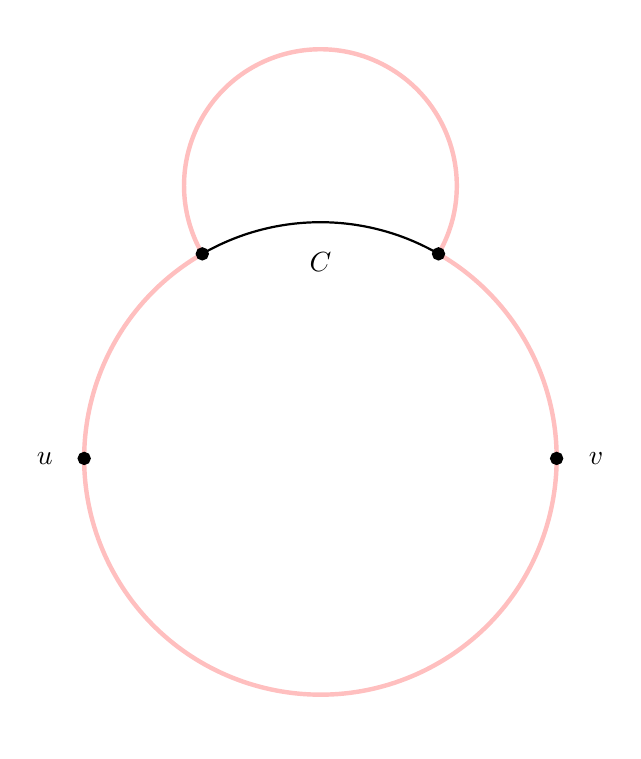
\begin{tikzpicture}
                \draw[pink, ultra thick] (1.5,{sqrt(27/4)}) arc (-30:210:{sqrt(3)});
                \draw[black, thick] (1.5,{sqrt(27/4)}) arc (60:120:3);
                \draw[pink, ultra thick] (-1.5,{sqrt(27/4)}) arc (120:420:3);
                \filldraw[black, thick] (1.5,{sqrt(27/4)}) circle (2pt);
                \filldraw[black, thick] (-1.5,{sqrt(27/4)}) circle (2pt);
                \filldraw[black, thick] (-3,0) circle (2pt);
                \filldraw[black, thick] (3,0) circle (2pt);

                \node at (-3.5,0,0) {$u$};
                \node at (3.5,0,0) {$v$};
                \node at (0,2.5,0) {$C$};
            \end{tikzpicture}
        \end{minipage}
        \hfill
        \begin{minipage}{0.4\textwidth}
            Ta không thể có extra paths ở phần trên hay dưới $C$ vì nó sẽ tạo ra chu trình chiếm nhiều diện tích hơn $C$, mâu thuẫn.
        \end{minipage}

    \end{figure}


    \begin{figure}[H]
        \begin{minipage}{0.4\textwidth}
            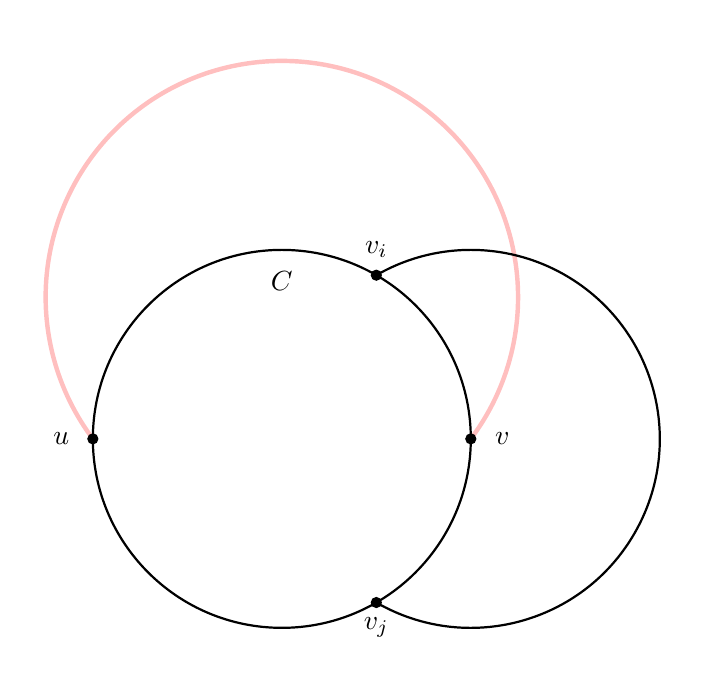
\begin{tikzpicture}[scale = 0.8]
                \draw[black, thick] (0,0) circle (3);
                \draw[pink, ultra thick] (3,0) arc (-acos(3/3.75):180+acos(3/3.75):3.75);
                \draw[black, thick] (1.5,-{sqrt(27/4)}) arc (-120:120:3);

                \filldraw[black, thick] (-3,0) circle (2pt);
                \filldraw[black, thick] (3,0) circle (2pt);
                \filldraw[black, thick] (1.5,{sqrt(27/4)}) circle (2pt);
                \filldraw[black, thick] (1.5,-{sqrt(27/4)}) circle (2pt);
                \node at (1.5,3,0) {$v_i$};
                \node at (1.5,-3,0) {$v_j$};
                \node at (-3.5,0,0) {$u$};
                \node at (3.5,0,0) {$v$};
                \node at (0,2.5,0) {$C$};
            \end{tikzpicture}
        \end{minipage}
        \hfill
        \begin{minipage}{0.4\textwidth}
            $G$ không phẳng, nên ta có một obstruction $uv$ ở phía ngoài của $C$. There must exist a path $v_iv_j$ that blocks $uv$
        \end{minipage}
    \end{figure}

    Phía trong của $C$ cũng cần có một obstruction. Cái obstruction này cũng phải block $v_iv_j$ và $uv$ from being draw inside of $C$ since otherwise we could just draw it inside and draw $uv$ on the outside.

    Tương đương, Ta có 4 loại obstructions tổng quát được miêu tả dưới đây. \\

    \begin{figure}[H]
        \begin{minipage}{0.4\textwidth}
            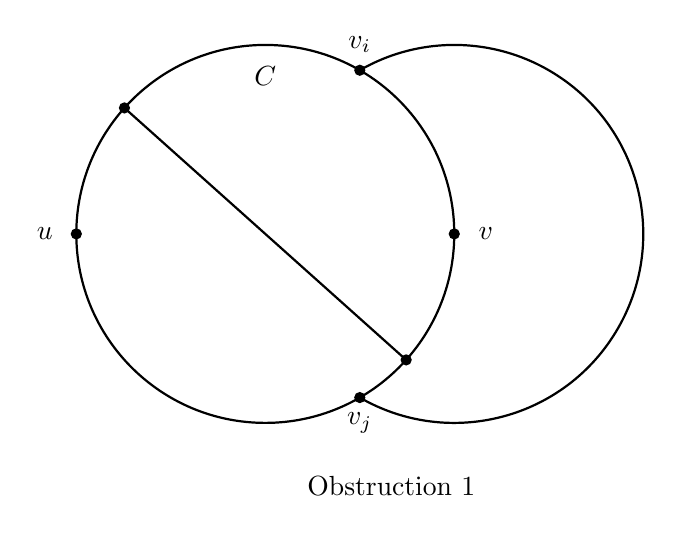
\begin{tikzpicture}[scale = 0.8]
                \draw[black, thick] (0,0) circle (3);
                \draw[black, thick] (1.5,-{sqrt(27/4)}) arc (-120:120:3);
                \draw[black, thick] ({-sqrt(5)},2) -- ({sqrt(5)},-2);
                \filldraw[black, thick] (-3,0) circle (2pt);
                \filldraw[black, thick] (3,0) circle (2pt);
                \filldraw[black, thick] ({-sqrt(5)},2) circle (2pt);
                \filldraw[black, thick] ({sqrt(5)},-2) circle (2pt);
                \filldraw[black, thick] (1.5,{sqrt(27/4)}) circle (2pt);
                \filldraw[black, thick] (1.5,-{sqrt(27/4)}) circle (2pt);
                \node at (1.5,3,0) {$v_i$};
                \node at (1.5,-3,0) {$v_j$};
                \node at (-3.5,0,0) {$u$};
                \node at (3.5,0,0) {$v$};
                \node at (0,2.5,0) {$C$};

                \node at (2,-4,0) {Obstruction 1};
            \end{tikzpicture}
        \end{minipage}
        \hfill
        \begin{minipage}{0.4\textwidth}
            \begin{tikzpicture}[scale = 0.8]
                \draw[black, thick] (0,0) circle (3);
                \draw[black, thick] (1.5,-{sqrt(27/4)}) arc (-120:120:3);
                \draw[black, thick] (3,0) arc (acos(0.6):180-acos(0.6):5);
                \draw[black, thick] ({sqrt(5)},-2) -- (-{sqrt(5)},2);
                \filldraw[blue, thick] (-3,0) circle (3pt);
                \filldraw[purple, thick] (3,0) circle (3pt);
                \filldraw[purple, thick] ({-sqrt(5)},2) circle (3pt);
                \filldraw[blue, thick] ({sqrt(5)},-2) circle (3pt);
                \filldraw[blue, thick] (1.5,{sqrt(27/4)}) circle (3pt);
                \filldraw[purple, thick] (1.5,-{sqrt(27/4)}) circle (3pt);
                \node at (1.5,3,0) {$v_i$};
                \node at (1.5,-3,0) {$v_j$};
                \node at (-3.5,0,0) {$u$};
                \node at (3.5,0,0) {$v$};
                \node at (0,2.5,0) {$C$};
                \node at (2,-4,0) {$G$ chứa một đồ thị phân chia của $K_{3,3}$};

            \end{tikzpicture}
        \end{minipage}
    \end{figure}

    \begin{figure}[H]
        \begin{minipage}{0.4\textwidth}
            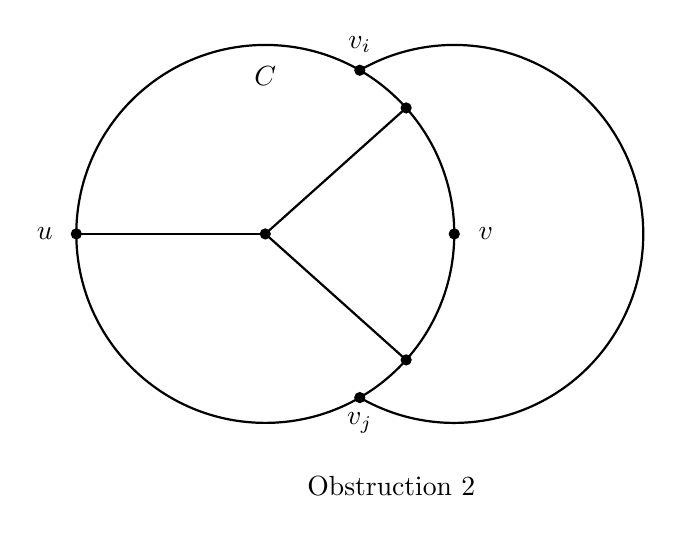
\begin{tikzpicture}[scale = 0.8]
                \draw[black, thick] (0,0) circle (3);
                \draw[black, thick] (1.5,-{sqrt(27/4)}) arc (-120:120:3);
                \draw[black, thick] (0,0) -- ({sqrt(5)},-2);
                \draw[black, thick] (0,0) -- ({sqrt(5)},2);
                \draw[black, thick] (0,0) -- (-3,0);
                \filldraw[black, thick] (-3,0) circle (2pt);
                \filldraw[black, thick] (3,0) circle (2pt);
                \filldraw[black, thick] (0,0) circle (2pt);
                \filldraw[black, thick] ({sqrt(5)},2) circle (2pt);
                \filldraw[black, thick] ({sqrt(5)},-2) circle (2pt);
                \filldraw[black, thick] (1.5,{sqrt(27/4)}) circle (2pt);
                \filldraw[black, thick] (1.5,-{sqrt(27/4)}) circle (2pt);
                \node at (1.5,3,0) {$v_i$};
                \node at (1.5,-3,0) {$v_j$};
                \node at (-3.5,0,0) {$u$};
                \node at (3.5,0,0) {$v$};
                \node at (0,2.5,0) {$C$};

                \node at (2,-4,0) {Obstruction 2};
            \end{tikzpicture}
        \end{minipage}
        \hfill
        \begin{minipage}{0.4\textwidth}
            \begin{tikzpicture}[scale = 0.8]
                \draw[black, thick] (0,0) circle (3);
                \draw[black, thick] (1.5,-{sqrt(27/4)}) arc (-120:120:3);
                \draw[black, thick] (3,0) arc (acos(0.6):180-acos(0.6):5);
                \draw[black, thick] (0,0) -- ({sqrt(5)},-2);
                \draw[black, thick] (0,0) -- ({sqrt(5)},2);
                \draw[black, thick] (0,0) -- (-3,0);
                \filldraw[blue, thick] (-3,0) circle (3pt);
                \filldraw[purple, thick] (3,0) circle (3pt);
                \filldraw[purple, thick] (0,0) circle (3pt);
                \filldraw[blue, thick] ({sqrt(5)},2) circle (3pt);
                \filldraw[blue, thick] ({sqrt(5)},-2) circle (3pt);
                \filldraw[black, thick] (1.5,{sqrt(27/4)}) circle (2pt);
                \filldraw[purple, thick] (1.5,-{sqrt(27/4)}) circle (3pt);
                \node at (1.5,3,0) {$v_i$};
                \node at (1.5,-3,0) {$v_j$};
                \node at (-3.5,0,0) {$u$};
                \node at (3.5,0,0) {$v$};
                \node at (0,2.5,0) {$C$};
                \node at (2,-4,0) {$G$ chứa một đồ thị phân chia của $K_{3,3}$};

            \end{tikzpicture}
        \end{minipage}
    \end{figure}

    \begin{figure}[H]
        \begin{minipage}{0.4\textwidth}
            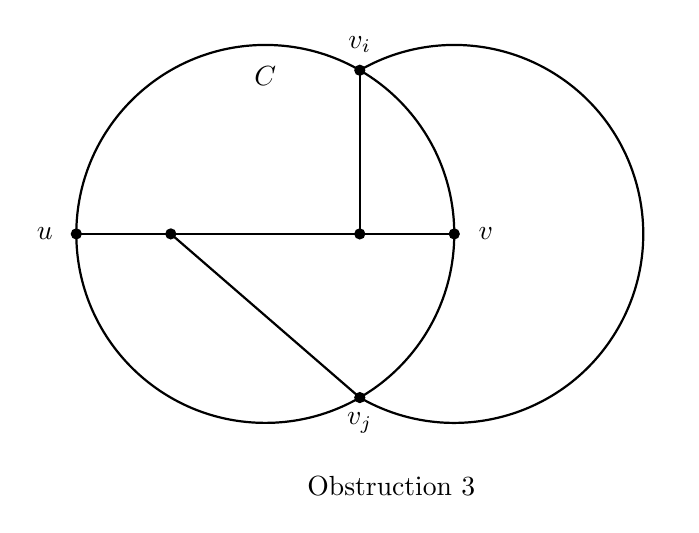
\begin{tikzpicture}[scale = 0.8]
                \draw[black, thick] (0,0) circle (3);
                \draw[black, thick] (1.5,-{sqrt(27/4)}) arc (-120:120:3);
                \draw[black, thick] (3,0) -- (-3,0);
                \draw[black, thick] (1.5,0) -- (1.5,{sqrt(27/4)});
                \draw[black, thick] (-1.5,0) -- (1.5,-{sqrt(27/4)});
                \filldraw[black, thick] (-3,0) circle (2pt);
                \filldraw[black, thick] (3,0) circle (2pt);
                \filldraw[black, thick] (1.5,{sqrt(27/4)}) circle (2pt);
                \filldraw[black, thick] (1.5,-{sqrt(27/4)}) circle (2pt);
                \filldraw[black, thick] (1.5,0) circle (2pt);
                \filldraw[black, thick] (-1.5,0) circle (2pt);
                \node at (1.5,3,0) {$v_i$};
                \node at (1.5,-3,0) {$v_j$};
                \node at (-3.5,0,0) {$u$};
                \node at (3.5,0,0) {$v$};
                \node at (0,2.5,0) {$C$};

                \node at (2,-4,0) {Obstruction 3};
            \end{tikzpicture}
        \end{minipage}
        \hfill
        \begin{minipage}{0.4\textwidth}
            \begin{tikzpicture}[scale = 0.8]
                \draw[black, thick] (3,0) arc (acos(0.6):180-acos(0.6):5);
                \draw[black, thick] (0,0) circle (3);
                \draw[black, thick] (1.5,-{sqrt(27/4)}) arc (-120:120:3);
                \draw[black, thick] (3,0) -- (-3,0);
                \draw[black, thick] (1.5,0) -- (1.5,{sqrt(27/4)});
                \draw[black, thick] (-1.5,0) -- (1.5,-{sqrt(27/4)});
                \filldraw[purple, thick] (-3,0) circle (3pt);
                \filldraw[blue, thick] (3,0) circle (3pt);
                \filldraw[blue, thick] (1.5,{sqrt(27/4)}) circle (3pt);
                \filldraw[purple, thick] (1.5,-{sqrt(27/4)}) circle (3pt);
                \filldraw[purple, thick] (1.5,0) circle (3pt);
                \filldraw[blue, thick] (-1.5,0) circle (3pt);
                \node at (1.5,3,0) {$v_i$};
                \node at (1.5,-3,0) {$v_j$};
                \node at (-3.5,0,0) {$u$};
                \node at (3.5,0,0) {$v$};
                \node at (0,2.5,0) {$C$};
                \node at (2,-4,0) {$G$ chứa một đồ thị phân chia của $K_{3,3}$};

            \end{tikzpicture}
        \end{minipage}
    \end{figure}


    \begin{figure}[H]
        \begin{minipage}{0.4\textwidth}
            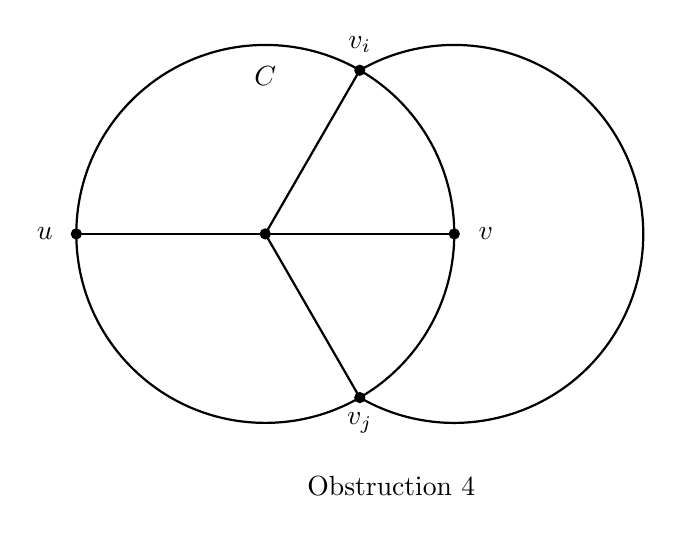
\begin{tikzpicture}[scale = 0.8]
                \draw[black, thick] (0,0) circle (3);
                \draw[black, thick] (1.5,-{sqrt(27/4)}) arc (-120:120:3);
                \draw[black, thick] (3,0) -- (-3,0);
                \draw[black, thick] (0,0) -- (1.5,{sqrt(27/4)});
                \draw[black, thick] (0,0) -- (1.5,-{sqrt(27/4)});
                \filldraw[black, thick] (-3,0) circle (2pt);
                \filldraw[black, thick] (3,0) circle (2pt);
                \filldraw[black, thick] (1.5,{sqrt(27/4)}) circle (2pt);
                \filldraw[black, thick] (1.5,-{sqrt(27/4)}) circle (2pt);
                \filldraw[black, thick] (0,0) circle (2pt);
                \node at (1.5,3,0) {$v_i$};
                \node at (1.5,-3,0) {$v_j$};
                \node at (-3.5,0,0) {$u$};
                \node at (3.5,0,0) {$v$};
                \node at (0,2.5,0) {$C$};

                \node at (2,-4,0) {Obstruction 4};
            \end{tikzpicture}
        \end{minipage}
        \hfill
        \begin{minipage}{0.4\textwidth}
            \begin{tikzpicture}[scale = 0.8]
                \draw[black, thick] (3,0) arc (acos(0.6):180-acos(0.6):5);
                \draw[black, thick] (0,0) circle (3);
                \draw[black, thick] (1.5,-{sqrt(27/4)}) arc (-120:120:3);
                \draw[black, thick] (3,0) -- (-3,0);
                \draw[black, thick] (0,0) -- (1.5,{sqrt(27/4)});
                \draw[black, thick] (0,0) -- (1.5,-{sqrt(27/4)});
                \filldraw[black, thick] (-3,0) circle (3pt);
                \filldraw[black, thick] (3,0) circle (3pt);
                \filldraw[black, thick] (1.5,{sqrt(27/4)}) circle (3pt);
                \filldraw[black, thick] (1.5,-{sqrt(27/4)}) circle (3pt);
                \filldraw[black, thick] (0,0) circle (3pt);
                \node at (1.5,3,0) {$v_i$};
                \node at (1.5,-3,0) {$v_j$};
                \node at (-3.5,0,0) {$u$};
                \node at (3.5,0,0) {$v$};
                \node at (0,2.5,0) {$C$};
                \node at (2,-4,0) {$G$ chứa một đồ thị phân chia của $K_5$};

            \end{tikzpicture}
        \end{minipage}
    \end{figure}
    \begin{remark}
        $G$ luôn có một đồ thị con là  đồ thị phân chia của $K_5$ hoặc $K_{3,3}$
    \end{remark}
    Kết quả của 4 trường hợp trên đều mâu thuẫn với giả thiết. Từ đây, ta kết luận rằng, không tồn tại đồ thị nào như $G$. Định lý được chứng minh.
\end{proof}


\section*{Acknowledgement}
\addcontentsline{toc}{section}{Acknowledgement}
Chúng tôi muốn gửi lời cảm ơn đến:
\begin{itemize}
    \item Người hướng dẫn, Nguyễn Hải Vinh, vì sự hướng dẫn.
    \item \href{https://cses.fi/book/book.pdf}{Giáo sư Antti Laaksonen} đã giới thiệu chúng tôi đến với Lý thuyết đồ thị.
    \item \href{https://www.youtube.com/channel/UCYO_jab_esuFRV4b17AJtAw}{3Blue1Brown} vì thư viện Python \href{https://github.com/dcabatin/manim}{manim}.
    \item \href{https://www.youtube.com/watch?v=DOnY6eZi2E8}{Nhóm của David Cabatingan} vì những lưu ý về \hyperref[thr:kuratowski]{Định lý Kuratowski}
    \item Ai đấy xây nên cái trường HUS.
\end{itemize}
\section*{Tài liệu tham khảo}
\addcontentsline{toc}{section}{Tài liệu tham khảo}
\end{document}